% Created by tikzDevice version 0.9 on 2016-01-12 22:38:37
% !TEX encoding = UTF-8 Unicode
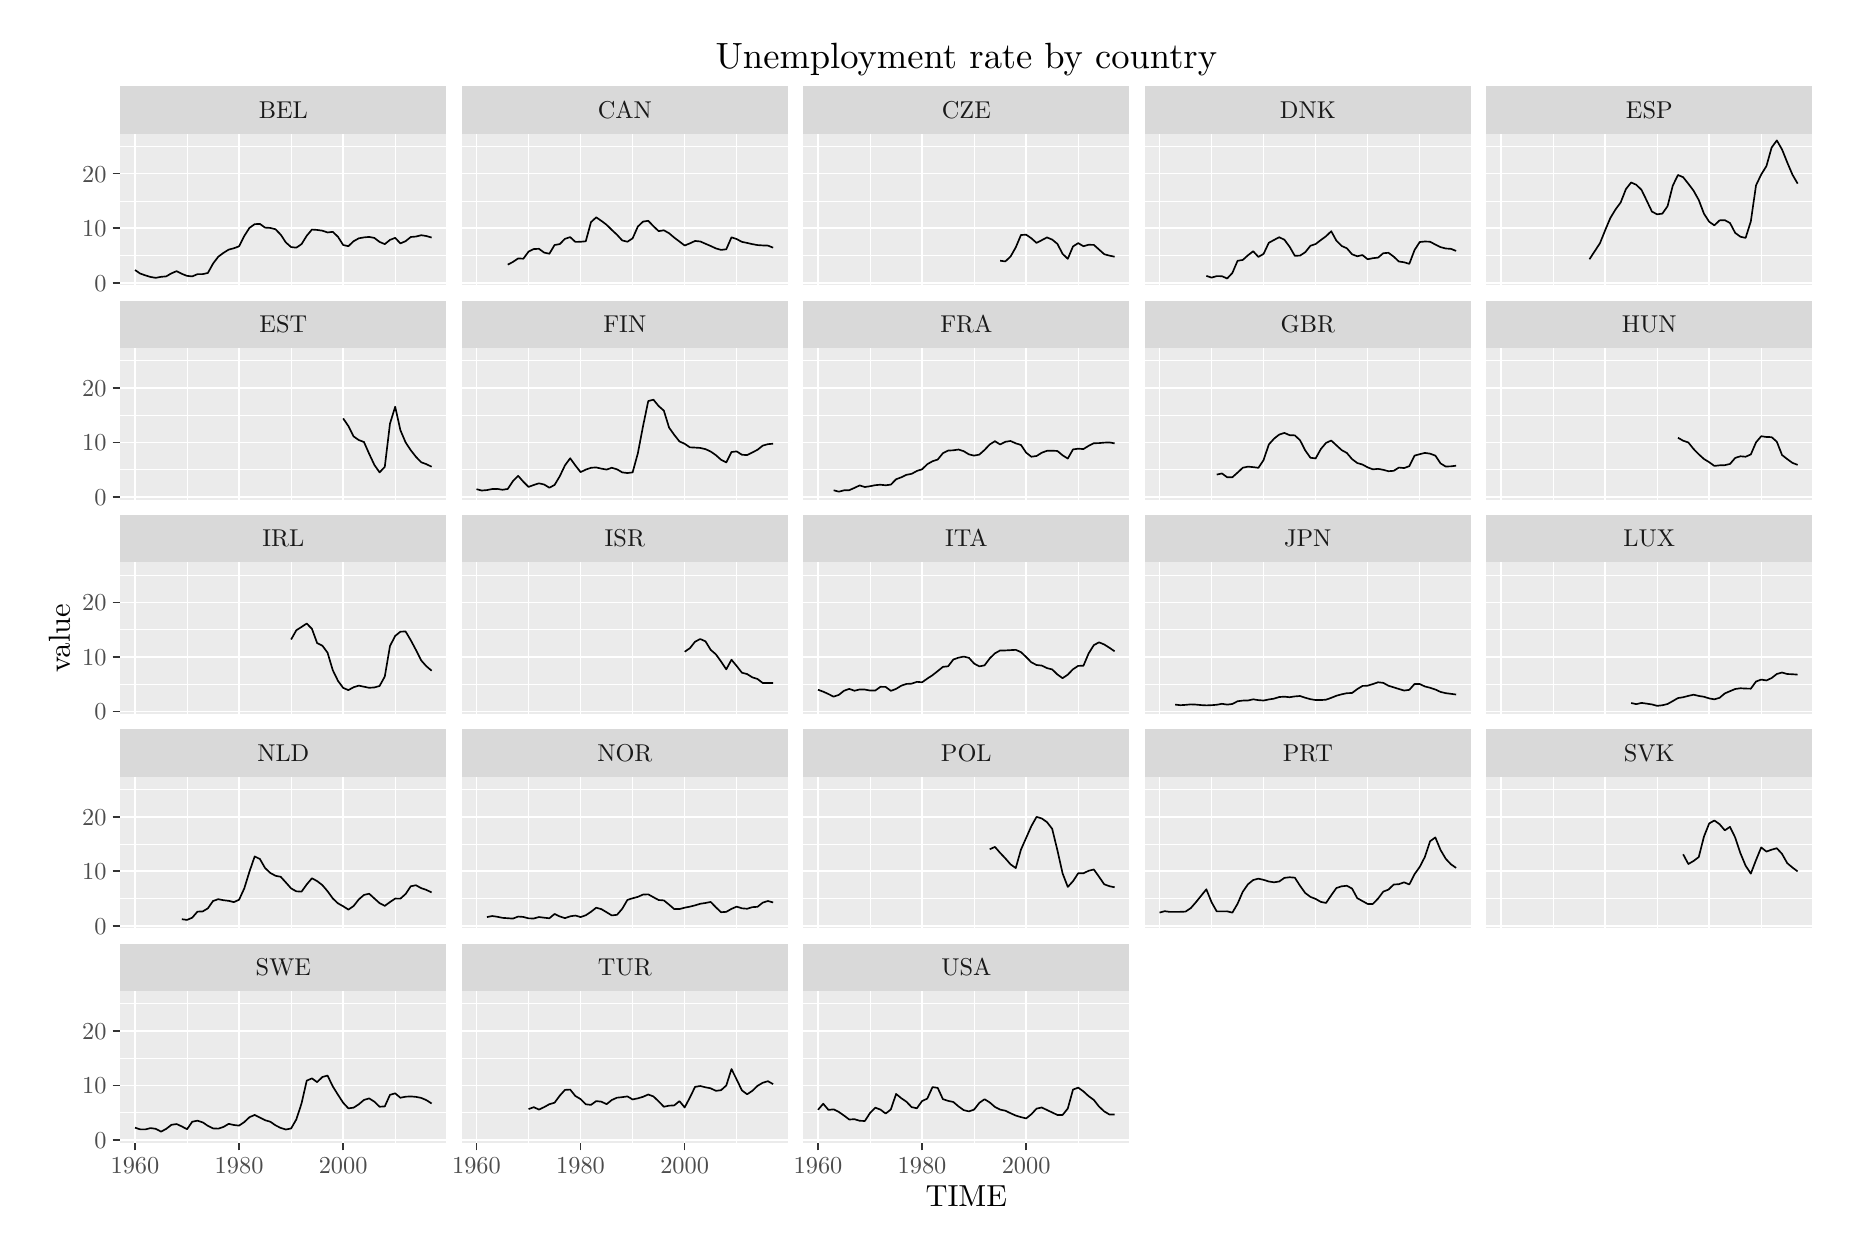
\begin{tikzpicture}[x=1pt,y=1pt]
\definecolor{fillColor}{RGB}{255,255,255}
\path[use as bounding box,fill=fillColor,fill opacity=0.00] (0,0) rectangle (650.43,433.62);
\begin{scope}
\path[clip] (  0.00,  0.00) rectangle (650.43,433.62);
\definecolor{drawColor}{RGB}{255,255,255}
\definecolor{fillColor}{RGB}{255,255,255}

\path[draw=drawColor,line width= 0.6pt,line join=round,line cap=round,fill=fillColor] (  0.00,  0.00) rectangle (650.43,433.62);
\end{scope}
\begin{scope}
\path[clip] ( 33.42,340.48) rectangle (151.33,395.37);
\definecolor{fillColor}{gray}{0.92}

\path[fill=fillColor] ( 33.42,340.48) rectangle (151.33,395.37);
\definecolor{drawColor}{RGB}{255,255,255}

\path[draw=drawColor,line width= 0.3pt,line join=round] ( 33.42,351.27) --
	(151.33,351.27);

\path[draw=drawColor,line width= 0.3pt,line join=round] ( 33.42,371.00) --
	(151.33,371.00);

\path[draw=drawColor,line width= 0.3pt,line join=round] ( 33.42,390.72) --
	(151.33,390.72);

\path[draw=drawColor,line width= 0.3pt,line join=round] ( 57.59,340.48) --
	( 57.59,395.37);

\path[draw=drawColor,line width= 0.3pt,line join=round] ( 95.20,340.48) --
	( 95.20,395.37);

\path[draw=drawColor,line width= 0.3pt,line join=round] (132.80,340.48) --
	(132.80,395.37);

\path[draw=drawColor,line width= 0.6pt,line join=round] ( 33.42,341.41) --
	(151.33,341.41);

\path[draw=drawColor,line width= 0.6pt,line join=round] ( 33.42,361.13) --
	(151.33,361.13);

\path[draw=drawColor,line width= 0.6pt,line join=round] ( 33.42,380.86) --
	(151.33,380.86);

\path[draw=drawColor,line width= 0.6pt,line join=round] ( 38.78,340.48) --
	( 38.78,395.37);

\path[draw=drawColor,line width= 0.6pt,line join=round] ( 76.39,340.48) --
	( 76.39,395.37);

\path[draw=drawColor,line width= 0.6pt,line join=round] (114.00,340.48) --
	(114.00,395.37);
\definecolor{drawColor}{RGB}{0,0,0}

\path[draw=drawColor,line width= 0.6pt,line join=round] ( 38.78,346.04) --
	( 40.66,344.76) --
	( 42.54,344.11) --
	( 44.42,343.53) --
	( 46.30,343.22) --
	( 48.19,343.58) --
	( 50.07,343.75) --
	( 51.95,344.85) --
	( 53.83,345.64) --
	( 55.71,344.66) --
	( 57.59,343.93) --
	( 59.47,343.74) --
	( 61.35,344.55) --
	( 63.23,344.57) --
	( 65.11,344.97) --
	( 66.99,348.37) --
	( 68.87,350.85) --
	( 70.75,352.24) --
	( 72.63,353.41) --
	( 74.51,353.91) --
	( 76.39,354.61) --
	( 78.27,358.34) --
	( 80.15,361.28) --
	( 82.03,362.61) --
	( 83.91,362.71) --
	( 85.79,361.36) --
	( 87.67,361.25) --
	( 89.55,360.77) --
	( 91.43,358.82) --
	( 93.31,355.99) --
	( 95.20,354.33) --
	( 97.08,354.12) --
	( 98.96,355.40) --
	(100.84,358.43) --
	(102.72,360.66) --
	(104.60,360.53) --
	(106.48,360.25) --
	(108.36,359.61) --
	(110.24,359.84) --
	(112.12,358.06) --
	(114.00,355.09) --
	(115.88,354.65) --
	(117.76,356.44) --
	(119.64,357.50) --
	(121.52,357.83) --
	(123.40,358.01) --
	(125.28,357.63) --
	(127.16,356.20) --
	(129.04,355.40) --
	(130.92,356.93) --
	(132.80,357.67) --
	(134.68,355.66) --
	(136.56,356.47) --
	(138.44,357.98) --
	(140.32,358.14) --
	(142.21,358.62) --
	(144.09,358.32) --
	(145.97,357.77);
\end{scope}
\begin{scope}
\path[clip] (156.83,340.48) rectangle (274.73,395.37);
\definecolor{fillColor}{gray}{0.92}

\path[fill=fillColor] (156.83,340.48) rectangle (274.73,395.37);
\definecolor{drawColor}{RGB}{255,255,255}

\path[draw=drawColor,line width= 0.3pt,line join=round] (156.83,351.27) --
	(274.73,351.27);

\path[draw=drawColor,line width= 0.3pt,line join=round] (156.83,371.00) --
	(274.73,371.00);

\path[draw=drawColor,line width= 0.3pt,line join=round] (156.83,390.72) --
	(274.73,390.72);

\path[draw=drawColor,line width= 0.3pt,line join=round] (180.99,340.48) --
	(180.99,395.37);

\path[draw=drawColor,line width= 0.3pt,line join=round] (218.60,340.48) --
	(218.60,395.37);

\path[draw=drawColor,line width= 0.3pt,line join=round] (256.20,340.48) --
	(256.20,395.37);

\path[draw=drawColor,line width= 0.6pt,line join=round] (156.83,341.41) --
	(274.73,341.41);

\path[draw=drawColor,line width= 0.6pt,line join=round] (156.83,361.13) --
	(274.73,361.13);

\path[draw=drawColor,line width= 0.6pt,line join=round] (156.83,380.86) --
	(274.73,380.86);

\path[draw=drawColor,line width= 0.6pt,line join=round] (162.18,340.48) --
	(162.18,395.37);

\path[draw=drawColor,line width= 0.6pt,line join=round] (199.79,340.48) --
	(199.79,395.37);

\path[draw=drawColor,line width= 0.6pt,line join=round] (237.40,340.48) --
	(237.40,395.37);
\definecolor{drawColor}{RGB}{0,0,0}

\path[draw=drawColor,line width= 0.6pt,line join=round] (173.47,347.99) --
	(175.35,348.96) --
	(177.23,350.24) --
	(179.11,350.13) --
	(180.99,352.69) --
	(182.87,353.62) --
	(184.75,353.71) --
	(186.63,352.34) --
	(188.51,351.93) --
	(190.39,355.08) --
	(192.27,355.41) --
	(194.15,357.32) --
	(196.03,357.93) --
	(197.91,356.20) --
	(199.79,356.25) --
	(201.67,356.43) --
	(203.55,363.35) --
	(205.43,365.07) --
	(207.31,363.81) --
	(209.19,362.39) --
	(211.07,360.53) --
	(212.96,358.78) --
	(214.84,356.73) --
	(216.72,356.27) --
	(218.60,357.49) --
	(220.48,361.75) --
	(222.36,363.54) --
	(224.24,363.83) --
	(226.12,361.88) --
	(228.00,360.09) --
	(229.88,360.40) --
	(231.76,359.34) --
	(233.64,357.75) --
	(235.52,356.33) --
	(237.40,354.90) --
	(239.28,355.67) --
	(241.16,356.54) --
	(243.04,356.36) --
	(244.92,355.53) --
	(246.80,354.73) --
	(248.68,353.85) --
	(250.56,353.31) --
	(252.44,353.54) --
	(254.32,357.87) --
	(256.20,357.23) --
	(258.08,356.22) --
	(259.97,355.83) --
	(261.85,355.40) --
	(263.73,355.05) --
	(265.61,354.93) --
	(267.49,354.87) --
	(269.37,354.12);
\end{scope}
\begin{scope}
\path[clip] (280.23,340.48) rectangle (398.13,395.37);
\definecolor{fillColor}{gray}{0.92}

\path[fill=fillColor] (280.23,340.48) rectangle (398.13,395.37);
\definecolor{drawColor}{RGB}{255,255,255}

\path[draw=drawColor,line width= 0.3pt,line join=round] (280.23,351.27) --
	(398.13,351.27);

\path[draw=drawColor,line width= 0.3pt,line join=round] (280.23,371.00) --
	(398.13,371.00);

\path[draw=drawColor,line width= 0.3pt,line join=round] (280.23,390.72) --
	(398.13,390.72);

\path[draw=drawColor,line width= 0.3pt,line join=round] (304.39,340.48) --
	(304.39,395.37);

\path[draw=drawColor,line width= 0.3pt,line join=round] (342.00,340.48) --
	(342.00,395.37);

\path[draw=drawColor,line width= 0.3pt,line join=round] (379.61,340.48) --
	(379.61,395.37);

\path[draw=drawColor,line width= 0.6pt,line join=round] (280.23,341.41) --
	(398.13,341.41);

\path[draw=drawColor,line width= 0.6pt,line join=round] (280.23,361.13) --
	(398.13,361.13);

\path[draw=drawColor,line width= 0.6pt,line join=round] (280.23,380.86) --
	(398.13,380.86);

\path[draw=drawColor,line width= 0.6pt,line join=round] (285.59,340.48) --
	(285.59,395.37);

\path[draw=drawColor,line width= 0.6pt,line join=round] (323.19,340.48) --
	(323.19,395.37);

\path[draw=drawColor,line width= 0.6pt,line join=round] (360.80,340.48) --
	(360.80,395.37);
\definecolor{drawColor}{RGB}{0,0,0}

\path[draw=drawColor,line width= 0.6pt,line join=round] (351.40,349.41) --
	(353.28,349.15) --
	(355.16,350.92) --
	(357.04,354.22) --
	(358.92,358.69) --
	(360.80,358.81) --
	(362.68,357.51) --
	(364.56,355.84) --
	(366.44,356.83) --
	(368.32,357.82) --
	(370.20,357.04) --
	(372.08,355.50) --
	(373.96,351.90) --
	(375.84,350.08) --
	(377.73,354.58) --
	(379.61,355.76) --
	(381.49,354.64) --
	(383.37,355.17) --
	(385.25,355.12) --
	(387.13,353.45) --
	(389.01,351.76) --
	(390.89,351.24) --
	(392.77,350.85);
\end{scope}
\begin{scope}
\path[clip] (403.63,340.48) rectangle (521.53,395.37);
\definecolor{fillColor}{gray}{0.92}

\path[fill=fillColor] (403.63,340.48) rectangle (521.53,395.37);
\definecolor{drawColor}{RGB}{255,255,255}

\path[draw=drawColor,line width= 0.3pt,line join=round] (403.63,351.27) --
	(521.53,351.27);

\path[draw=drawColor,line width= 0.3pt,line join=round] (403.63,371.00) --
	(521.53,371.00);

\path[draw=drawColor,line width= 0.3pt,line join=round] (403.63,390.72) --
	(521.53,390.72);

\path[draw=drawColor,line width= 0.3pt,line join=round] (427.79,340.48) --
	(427.79,395.37);

\path[draw=drawColor,line width= 0.3pt,line join=round] (465.40,340.48) --
	(465.40,395.37);

\path[draw=drawColor,line width= 0.3pt,line join=round] (503.01,340.48) --
	(503.01,395.37);

\path[draw=drawColor,line width= 0.6pt,line join=round] (403.63,341.41) --
	(521.53,341.41);

\path[draw=drawColor,line width= 0.6pt,line join=round] (403.63,361.13) --
	(521.53,361.13);

\path[draw=drawColor,line width= 0.6pt,line join=round] (403.63,380.86) --
	(521.53,380.86);

\path[draw=drawColor,line width= 0.6pt,line join=round] (408.99,340.48) --
	(408.99,395.37);

\path[draw=drawColor,line width= 0.6pt,line join=round] (446.59,340.48) --
	(446.59,395.37);

\path[draw=drawColor,line width= 0.6pt,line join=round] (484.20,340.48) --
	(484.20,395.37);
\definecolor{drawColor}{RGB}{0,0,0}

\path[draw=drawColor,line width= 0.6pt,line join=round] (425.91,343.92) --
	(427.79,343.31) --
	(429.67,343.84) --
	(431.55,343.81) --
	(433.43,342.98) --
	(435.31,344.98) --
	(437.19,349.38) --
	(439.07,349.68) --
	(440.95,351.37) --
	(442.83,352.83) --
	(444.71,350.78) --
	(446.59,351.88) --
	(448.48,355.88) --
	(450.36,356.90) --
	(452.24,357.90) --
	(454.12,356.98) --
	(456.00,354.45) --
	(457.88,351.17) --
	(459.76,351.26) --
	(461.64,352.46) --
	(463.52,354.80) --
	(465.40,355.44) --
	(467.28,356.87) --
	(469.16,358.25) --
	(471.04,360.06) --
	(472.92,356.61) --
	(474.80,354.74) --
	(476.68,353.90) --
	(478.56,351.73) --
	(480.44,351.01) --
	(482.32,351.45) --
	(484.20,349.93) --
	(486.08,350.32) --
	(487.96,350.52) --
	(489.84,352.12) --
	(491.72,352.27) --
	(493.60,350.89) --
	(495.49,349.11) --
	(497.37,348.84) --
	(499.25,348.27) --
	(501.13,353.24) --
	(503.01,356.16) --
	(504.89,356.35) --
	(506.77,356.26) --
	(508.65,355.24) --
	(510.53,354.32) --
	(512.41,353.82) --
	(514.29,353.69) --
	(516.17,352.95);
\end{scope}
\begin{scope}
\path[clip] (527.03,340.48) rectangle (644.93,395.37);
\definecolor{fillColor}{gray}{0.92}

\path[fill=fillColor] (527.03,340.48) rectangle (644.93,395.37);
\definecolor{drawColor}{RGB}{255,255,255}

\path[draw=drawColor,line width= 0.3pt,line join=round] (527.03,351.27) --
	(644.93,351.27);

\path[draw=drawColor,line width= 0.3pt,line join=round] (527.03,371.00) --
	(644.93,371.00);

\path[draw=drawColor,line width= 0.3pt,line join=round] (527.03,390.72) --
	(644.93,390.72);

\path[draw=drawColor,line width= 0.3pt,line join=round] (551.19,340.48) --
	(551.19,395.37);

\path[draw=drawColor,line width= 0.3pt,line join=round] (588.80,340.48) --
	(588.80,395.37);

\path[draw=drawColor,line width= 0.3pt,line join=round] (626.41,340.48) --
	(626.41,395.37);

\path[draw=drawColor,line width= 0.6pt,line join=round] (527.03,341.41) --
	(644.93,341.41);

\path[draw=drawColor,line width= 0.6pt,line join=round] (527.03,361.13) --
	(644.93,361.13);

\path[draw=drawColor,line width= 0.6pt,line join=round] (527.03,380.86) --
	(644.93,380.86);

\path[draw=drawColor,line width= 0.6pt,line join=round] (532.39,340.48) --
	(532.39,395.37);

\path[draw=drawColor,line width= 0.6pt,line join=round] (570.00,340.48) --
	(570.00,395.37);

\path[draw=drawColor,line width= 0.6pt,line join=round] (607.60,340.48) --
	(607.60,395.37);
\definecolor{drawColor}{RGB}{0,0,0}

\path[draw=drawColor,line width= 0.6pt,line join=round] (564.35,349.93) --
	(566.24,352.84) --
	(568.12,355.68) --
	(570.00,360.37) --
	(571.88,364.82) --
	(573.76,367.93) --
	(575.64,370.49) --
	(577.52,375.28) --
	(579.40,377.68) --
	(581.28,376.84) --
	(583.16,374.99) --
	(585.04,371.11) --
	(586.92,367.15) --
	(588.80,366.17) --
	(590.68,366.42) --
	(592.56,369.09) --
	(594.44,376.49) --
	(596.32,380.38) --
	(598.20,379.58) --
	(600.08,377.21) --
	(601.96,374.72) --
	(603.84,371.34) --
	(605.72,366.40) --
	(607.60,363.49) --
	(609.48,362.18) --
	(611.36,363.99) --
	(613.25,364.06) --
	(615.13,363.03) --
	(617.01,359.45) --
	(618.89,358.08) --
	(620.77,357.65) --
	(622.65,363.61) --
	(624.53,376.63) --
	(626.41,380.58) --
	(628.29,383.60) --
	(630.17,390.30) --
	(632.05,392.87) --
	(633.93,389.61) --
	(635.81,384.92) --
	(637.69,380.51) --
	(639.57,377.27);
\end{scope}
\begin{scope}
\path[clip] ( 33.42,263.03) rectangle (151.33,317.92);
\definecolor{fillColor}{gray}{0.92}

\path[fill=fillColor] ( 33.42,263.03) rectangle (151.33,317.92);
\definecolor{drawColor}{RGB}{255,255,255}

\path[draw=drawColor,line width= 0.3pt,line join=round] ( 33.42,273.83) --
	(151.33,273.83);

\path[draw=drawColor,line width= 0.3pt,line join=round] ( 33.42,293.55) --
	(151.33,293.55);

\path[draw=drawColor,line width= 0.3pt,line join=round] ( 33.42,313.27) --
	(151.33,313.27);

\path[draw=drawColor,line width= 0.3pt,line join=round] ( 57.59,263.03) --
	( 57.59,317.92);

\path[draw=drawColor,line width= 0.3pt,line join=round] ( 95.20,263.03) --
	( 95.20,317.92);

\path[draw=drawColor,line width= 0.3pt,line join=round] (132.80,263.03) --
	(132.80,317.92);

\path[draw=drawColor,line width= 0.6pt,line join=round] ( 33.42,263.96) --
	(151.33,263.96);

\path[draw=drawColor,line width= 0.6pt,line join=round] ( 33.42,283.69) --
	(151.33,283.69);

\path[draw=drawColor,line width= 0.6pt,line join=round] ( 33.42,303.41) --
	(151.33,303.41);

\path[draw=drawColor,line width= 0.6pt,line join=round] ( 38.78,263.03) --
	( 38.78,317.92);

\path[draw=drawColor,line width= 0.6pt,line join=round] ( 76.39,263.03) --
	( 76.39,317.92);

\path[draw=drawColor,line width= 0.6pt,line join=round] (114.00,263.03) --
	(114.00,317.92);
\definecolor{drawColor}{RGB}{0,0,0}

\path[draw=drawColor,line width= 0.6pt,line join=round] (114.00,292.41) --
	(115.88,289.67) --
	(117.76,285.92) --
	(119.64,284.61) --
	(121.52,283.89) --
	(123.40,279.63) --
	(125.28,275.61) --
	(127.16,272.92) --
	(129.04,274.92) --
	(130.92,290.54) --
	(132.80,296.64) --
	(134.68,288.17) --
	(136.56,283.76) --
	(138.44,280.92) --
	(140.32,278.52) --
	(142.21,276.57) --
	(144.09,275.88) --
	(145.97,274.96);
\end{scope}
\begin{scope}
\path[clip] (156.83,263.03) rectangle (274.73,317.92);
\definecolor{fillColor}{gray}{0.92}

\path[fill=fillColor] (156.83,263.03) rectangle (274.73,317.92);
\definecolor{drawColor}{RGB}{255,255,255}

\path[draw=drawColor,line width= 0.3pt,line join=round] (156.83,273.83) --
	(274.73,273.83);

\path[draw=drawColor,line width= 0.3pt,line join=round] (156.83,293.55) --
	(274.73,293.55);

\path[draw=drawColor,line width= 0.3pt,line join=round] (156.83,313.27) --
	(274.73,313.27);

\path[draw=drawColor,line width= 0.3pt,line join=round] (180.99,263.03) --
	(180.99,317.92);

\path[draw=drawColor,line width= 0.3pt,line join=round] (218.60,263.03) --
	(218.60,317.92);

\path[draw=drawColor,line width= 0.3pt,line join=round] (256.20,263.03) --
	(256.20,317.92);

\path[draw=drawColor,line width= 0.6pt,line join=round] (156.83,263.96) --
	(274.73,263.96);

\path[draw=drawColor,line width= 0.6pt,line join=round] (156.83,283.69) --
	(274.73,283.69);

\path[draw=drawColor,line width= 0.6pt,line join=round] (156.83,303.41) --
	(274.73,303.41);

\path[draw=drawColor,line width= 0.6pt,line join=round] (162.18,263.03) --
	(162.18,317.92);

\path[draw=drawColor,line width= 0.6pt,line join=round] (199.79,263.03) --
	(199.79,317.92);

\path[draw=drawColor,line width= 0.6pt,line join=round] (237.40,263.03) --
	(237.40,317.92);
\definecolor{drawColor}{RGB}{0,0,0}

\path[draw=drawColor,line width= 0.6pt,line join=round] (162.18,266.85) --
	(164.06,266.36) --
	(165.95,266.53) --
	(167.83,266.90) --
	(169.71,266.95) --
	(171.59,266.64) --
	(173.47,266.94) --
	(175.35,269.76) --
	(177.23,271.68) --
	(179.11,269.54) --
	(180.99,267.68) --
	(182.87,268.36) --
	(184.75,268.97) --
	(186.63,268.54) --
	(188.51,267.38) --
	(190.39,268.38) --
	(192.27,271.52) --
	(194.15,275.46) --
	(196.03,278.02) --
	(197.91,275.42) --
	(199.79,273.02) --
	(201.67,273.92) --
	(203.55,274.58) --
	(205.43,274.71) --
	(207.31,274.27) --
	(209.19,273.94) --
	(211.07,274.59) --
	(212.96,274.03) --
	(214.84,272.92) --
	(216.72,272.68) --
	(218.60,272.92) --
	(220.48,279.80) --
	(222.36,289.64) --
	(224.24,298.69) --
	(226.12,299.19) --
	(228.00,296.88) --
	(229.88,295.24) --
	(231.76,289.12) --
	(233.64,286.47) --
	(235.52,284.10) --
	(237.40,283.26) --
	(239.28,281.97) --
	(241.16,281.88) --
	(243.04,281.75) --
	(244.92,281.32) --
	(246.80,280.46) --
	(248.68,279.15) --
	(250.56,277.47) --
	(252.44,276.52) --
	(254.32,280.28) --
	(256.20,280.50) --
	(258.08,279.30) --
	(259.97,279.16) --
	(261.85,280.13) --
	(263.73,281.09) --
	(265.61,282.59) --
	(267.49,283.12) --
	(269.37,283.28);
\end{scope}
\begin{scope}
\path[clip] (280.23,263.03) rectangle (398.13,317.92);
\definecolor{fillColor}{gray}{0.92}

\path[fill=fillColor] (280.23,263.03) rectangle (398.13,317.92);
\definecolor{drawColor}{RGB}{255,255,255}

\path[draw=drawColor,line width= 0.3pt,line join=round] (280.23,273.83) --
	(398.13,273.83);

\path[draw=drawColor,line width= 0.3pt,line join=round] (280.23,293.55) --
	(398.13,293.55);

\path[draw=drawColor,line width= 0.3pt,line join=round] (280.23,313.27) --
	(398.13,313.27);

\path[draw=drawColor,line width= 0.3pt,line join=round] (304.39,263.03) --
	(304.39,317.92);

\path[draw=drawColor,line width= 0.3pt,line join=round] (342.00,263.03) --
	(342.00,317.92);

\path[draw=drawColor,line width= 0.3pt,line join=round] (379.61,263.03) --
	(379.61,317.92);

\path[draw=drawColor,line width= 0.6pt,line join=round] (280.23,263.96) --
	(398.13,263.96);

\path[draw=drawColor,line width= 0.6pt,line join=round] (280.23,283.69) --
	(398.13,283.69);

\path[draw=drawColor,line width= 0.6pt,line join=round] (280.23,303.41) --
	(398.13,303.41);

\path[draw=drawColor,line width= 0.6pt,line join=round] (285.59,263.03) --
	(285.59,317.92);

\path[draw=drawColor,line width= 0.6pt,line join=round] (323.19,263.03) --
	(323.19,317.92);

\path[draw=drawColor,line width= 0.6pt,line join=round] (360.80,263.03) --
	(360.80,317.92);
\definecolor{drawColor}{RGB}{0,0,0}

\path[draw=drawColor,line width= 0.6pt,line join=round] (291.23,266.46) --
	(293.11,265.95) --
	(294.99,266.44) --
	(296.87,266.49) --
	(298.75,267.32) --
	(300.63,268.21) --
	(302.51,267.63) --
	(304.39,267.92) --
	(306.27,268.30) --
	(308.15,268.46) --
	(310.03,268.26) --
	(311.91,268.50) --
	(313.79,270.43) --
	(315.67,271.14) --
	(317.55,272.04) --
	(319.43,272.40) --
	(321.31,273.43) --
	(323.19,274.04) --
	(325.07,275.88) --
	(326.95,276.94) --
	(328.83,277.55) --
	(330.72,279.85) --
	(332.60,280.80) --
	(334.48,280.90) --
	(336.36,281.18) --
	(338.24,280.58) --
	(340.12,279.42) --
	(342.00,278.98) --
	(343.88,279.35) --
	(345.76,281.03) --
	(347.64,283.01) --
	(349.52,284.19) --
	(351.40,283.00) --
	(353.28,283.98) --
	(355.16,284.26) --
	(357.04,283.42) --
	(358.92,282.83) --
	(360.80,280.05) --
	(362.68,278.57) --
	(364.56,278.84) --
	(366.44,280.02) --
	(368.32,280.72) --
	(370.20,280.75) --
	(372.08,280.66) --
	(373.96,279.10) --
	(375.84,277.91) --
	(377.73,281.23) --
	(379.61,281.48) --
	(381.49,281.35) --
	(383.37,282.51) --
	(385.25,283.45) --
	(387.13,283.50) --
	(389.01,283.67) --
	(390.89,283.75) --
	(392.77,283.40);
\end{scope}
\begin{scope}
\path[clip] (403.63,263.03) rectangle (521.53,317.92);
\definecolor{fillColor}{gray}{0.92}

\path[fill=fillColor] (403.63,263.03) rectangle (521.53,317.92);
\definecolor{drawColor}{RGB}{255,255,255}

\path[draw=drawColor,line width= 0.3pt,line join=round] (403.63,273.83) --
	(521.53,273.83);

\path[draw=drawColor,line width= 0.3pt,line join=round] (403.63,293.55) --
	(521.53,293.55);

\path[draw=drawColor,line width= 0.3pt,line join=round] (403.63,313.27) --
	(521.53,313.27);

\path[draw=drawColor,line width= 0.3pt,line join=round] (427.79,263.03) --
	(427.79,317.92);

\path[draw=drawColor,line width= 0.3pt,line join=round] (465.40,263.03) --
	(465.40,317.92);

\path[draw=drawColor,line width= 0.3pt,line join=round] (503.01,263.03) --
	(503.01,317.92);

\path[draw=drawColor,line width= 0.6pt,line join=round] (403.63,263.96) --
	(521.53,263.96);

\path[draw=drawColor,line width= 0.6pt,line join=round] (403.63,283.69) --
	(521.53,283.69);

\path[draw=drawColor,line width= 0.6pt,line join=round] (403.63,303.41) --
	(521.53,303.41);

\path[draw=drawColor,line width= 0.6pt,line join=round] (408.99,263.03) --
	(408.99,317.92);

\path[draw=drawColor,line width= 0.6pt,line join=round] (446.59,263.03) --
	(446.59,317.92);

\path[draw=drawColor,line width= 0.6pt,line join=round] (484.20,263.03) --
	(484.20,317.92);
\definecolor{drawColor}{RGB}{0,0,0}

\path[draw=drawColor,line width= 0.6pt,line join=round] (429.67,272.13) --
	(431.55,272.53) --
	(433.43,271.16) --
	(435.31,271.17) --
	(437.19,272.83) --
	(439.07,274.60) --
	(440.95,275.00) --
	(442.83,274.82) --
	(444.71,274.57) --
	(446.59,277.39) --
	(448.48,282.99) --
	(450.36,285.10) --
	(452.24,286.59) --
	(454.12,287.18) --
	(456.00,286.36) --
	(457.88,286.30) --
	(459.76,284.54) --
	(461.64,280.87) --
	(463.52,278.21) --
	(465.40,277.96) --
	(467.28,281.35) --
	(469.16,283.58) --
	(471.04,284.43) --
	(472.92,282.69) --
	(474.80,280.97) --
	(476.68,279.94) --
	(478.56,277.71) --
	(480.44,276.30) --
	(482.32,275.76) --
	(484.20,274.73) --
	(486.08,274.02) --
	(487.96,274.20) --
	(489.84,273.85) --
	(491.72,273.34) --
	(493.60,273.49) --
	(495.49,274.66) --
	(497.37,274.48) --
	(499.25,275.18) --
	(501.13,278.98) --
	(503.01,279.49) --
	(504.89,279.96) --
	(506.77,279.68) --
	(508.65,278.98) --
	(510.53,276.17) --
	(512.41,275.03) --
	(514.29,275.11) --
	(516.17,275.33);
\end{scope}
\begin{scope}
\path[clip] (527.03,263.03) rectangle (644.93,317.92);
\definecolor{fillColor}{gray}{0.92}

\path[fill=fillColor] (527.03,263.03) rectangle (644.93,317.92);
\definecolor{drawColor}{RGB}{255,255,255}

\path[draw=drawColor,line width= 0.3pt,line join=round] (527.03,273.83) --
	(644.93,273.83);

\path[draw=drawColor,line width= 0.3pt,line join=round] (527.03,293.55) --
	(644.93,293.55);

\path[draw=drawColor,line width= 0.3pt,line join=round] (527.03,313.27) --
	(644.93,313.27);

\path[draw=drawColor,line width= 0.3pt,line join=round] (551.19,263.03) --
	(551.19,317.92);

\path[draw=drawColor,line width= 0.3pt,line join=round] (588.80,263.03) --
	(588.80,317.92);

\path[draw=drawColor,line width= 0.3pt,line join=round] (626.41,263.03) --
	(626.41,317.92);

\path[draw=drawColor,line width= 0.6pt,line join=round] (527.03,263.96) --
	(644.93,263.96);

\path[draw=drawColor,line width= 0.6pt,line join=round] (527.03,283.69) --
	(644.93,283.69);

\path[draw=drawColor,line width= 0.6pt,line join=round] (527.03,303.41) --
	(644.93,303.41);

\path[draw=drawColor,line width= 0.6pt,line join=round] (532.39,263.03) --
	(532.39,317.92);

\path[draw=drawColor,line width= 0.6pt,line join=round] (570.00,263.03) --
	(570.00,317.92);

\path[draw=drawColor,line width= 0.6pt,line join=round] (607.60,263.03) --
	(607.60,317.92);
\definecolor{drawColor}{RGB}{0,0,0}

\path[draw=drawColor,line width= 0.6pt,line join=round] (596.32,285.44) --
	(598.20,284.37) --
	(600.08,283.73) --
	(601.96,281.38) --
	(603.84,279.46) --
	(605.72,277.75) --
	(607.60,276.61) --
	(609.48,275.26) --
	(611.36,275.47) --
	(613.25,275.53) --
	(615.13,275.96) --
	(617.01,278.15) --
	(618.89,278.74) --
	(620.77,278.58) --
	(622.65,279.40) --
	(624.53,283.77) --
	(626.41,285.99) --
	(628.29,285.71) --
	(630.17,285.66) --
	(632.05,284.00) --
	(633.93,279.20) --
	(635.81,277.72) --
	(637.69,276.36) --
	(639.57,275.63);
\end{scope}
\begin{scope}
\path[clip] ( 33.42,185.58) rectangle (151.33,240.47);
\definecolor{fillColor}{gray}{0.92}

\path[fill=fillColor] ( 33.42,185.58) rectangle (151.33,240.47);
\definecolor{drawColor}{RGB}{255,255,255}

\path[draw=drawColor,line width= 0.3pt,line join=round] ( 33.42,196.38) --
	(151.33,196.38);

\path[draw=drawColor,line width= 0.3pt,line join=round] ( 33.42,216.10) --
	(151.33,216.10);

\path[draw=drawColor,line width= 0.3pt,line join=round] ( 33.42,235.82) --
	(151.33,235.82);

\path[draw=drawColor,line width= 0.3pt,line join=round] ( 57.59,185.58) --
	( 57.59,240.47);

\path[draw=drawColor,line width= 0.3pt,line join=round] ( 95.20,185.58) --
	( 95.20,240.47);

\path[draw=drawColor,line width= 0.3pt,line join=round] (132.80,185.58) --
	(132.80,240.47);

\path[draw=drawColor,line width= 0.6pt,line join=round] ( 33.42,186.52) --
	(151.33,186.52);

\path[draw=drawColor,line width= 0.6pt,line join=round] ( 33.42,206.24) --
	(151.33,206.24);

\path[draw=drawColor,line width= 0.6pt,line join=round] ( 33.42,225.96) --
	(151.33,225.96);

\path[draw=drawColor,line width= 0.6pt,line join=round] ( 38.78,185.58) --
	( 38.78,240.47);

\path[draw=drawColor,line width= 0.6pt,line join=round] ( 76.39,185.58) --
	( 76.39,240.47);

\path[draw=drawColor,line width= 0.6pt,line join=round] (114.00,185.58) --
	(114.00,240.47);
\definecolor{drawColor}{RGB}{0,0,0}

\path[draw=drawColor,line width= 0.6pt,line join=round] ( 95.20,212.54) --
	( 97.08,215.88) --
	( 98.96,217.07) --
	(100.84,218.31) --
	(102.72,216.38) --
	(104.60,211.22) --
	(106.48,210.32) --
	(108.36,207.77) --
	(110.24,201.47) --
	(112.12,197.60) --
	(114.00,195.05) --
	(115.88,194.24) --
	(117.76,195.28) --
	(119.64,195.87) --
	(121.52,195.47) --
	(123.40,195.08) --
	(125.28,195.21) --
	(127.16,195.74) --
	(129.04,199.15) --
	(130.92,210.18) --
	(132.80,213.83) --
	(134.68,215.35) --
	(136.56,215.44) --
	(138.44,212.25) --
	(140.32,208.72) --
	(142.21,204.96) --
	(144.09,202.85) --
	(145.97,201.26);
\end{scope}
\begin{scope}
\path[clip] (156.83,185.58) rectangle (274.73,240.47);
\definecolor{fillColor}{gray}{0.92}

\path[fill=fillColor] (156.83,185.58) rectangle (274.73,240.47);
\definecolor{drawColor}{RGB}{255,255,255}

\path[draw=drawColor,line width= 0.3pt,line join=round] (156.83,196.38) --
	(274.73,196.38);

\path[draw=drawColor,line width= 0.3pt,line join=round] (156.83,216.10) --
	(274.73,216.10);

\path[draw=drawColor,line width= 0.3pt,line join=round] (156.83,235.82) --
	(274.73,235.82);

\path[draw=drawColor,line width= 0.3pt,line join=round] (180.99,185.58) --
	(180.99,240.47);

\path[draw=drawColor,line width= 0.3pt,line join=round] (218.60,185.58) --
	(218.60,240.47);

\path[draw=drawColor,line width= 0.3pt,line join=round] (256.20,185.58) --
	(256.20,240.47);

\path[draw=drawColor,line width= 0.6pt,line join=round] (156.83,186.52) --
	(274.73,186.52);

\path[draw=drawColor,line width= 0.6pt,line join=round] (156.83,206.24) --
	(274.73,206.24);

\path[draw=drawColor,line width= 0.6pt,line join=round] (156.83,225.96) --
	(274.73,225.96);

\path[draw=drawColor,line width= 0.6pt,line join=round] (162.18,185.58) --
	(162.18,240.47);

\path[draw=drawColor,line width= 0.6pt,line join=round] (199.79,185.58) --
	(199.79,240.47);

\path[draw=drawColor,line width= 0.6pt,line join=round] (237.40,185.58) --
	(237.40,240.47);
\definecolor{drawColor}{RGB}{0,0,0}

\path[draw=drawColor,line width= 0.6pt,line join=round] (237.40,208.11) --
	(239.28,209.38) --
	(241.16,211.74) --
	(243.04,212.71) --
	(244.92,211.87) --
	(246.80,208.80) --
	(248.68,207.18) --
	(250.56,204.56) --
	(252.44,201.76) --
	(254.32,205.21) --
	(256.20,202.96) --
	(258.08,200.54) --
	(259.97,200.04) --
	(261.85,198.86) --
	(263.73,198.26) --
	(265.61,196.81) --
	(267.49,196.81) --
	(269.37,196.81);
\end{scope}
\begin{scope}
\path[clip] (280.23,185.58) rectangle (398.13,240.47);
\definecolor{fillColor}{gray}{0.92}

\path[fill=fillColor] (280.23,185.58) rectangle (398.13,240.47);
\definecolor{drawColor}{RGB}{255,255,255}

\path[draw=drawColor,line width= 0.3pt,line join=round] (280.23,196.38) --
	(398.13,196.38);

\path[draw=drawColor,line width= 0.3pt,line join=round] (280.23,216.10) --
	(398.13,216.10);

\path[draw=drawColor,line width= 0.3pt,line join=round] (280.23,235.82) --
	(398.13,235.82);

\path[draw=drawColor,line width= 0.3pt,line join=round] (304.39,185.58) --
	(304.39,240.47);

\path[draw=drawColor,line width= 0.3pt,line join=round] (342.00,185.58) --
	(342.00,240.47);

\path[draw=drawColor,line width= 0.3pt,line join=round] (379.61,185.58) --
	(379.61,240.47);

\path[draw=drawColor,line width= 0.6pt,line join=round] (280.23,186.52) --
	(398.13,186.52);

\path[draw=drawColor,line width= 0.6pt,line join=round] (280.23,206.24) --
	(398.13,206.24);

\path[draw=drawColor,line width= 0.6pt,line join=round] (280.23,225.96) --
	(398.13,225.96);

\path[draw=drawColor,line width= 0.6pt,line join=round] (285.59,185.58) --
	(285.59,240.47);

\path[draw=drawColor,line width= 0.6pt,line join=round] (323.19,185.58) --
	(323.19,240.47);

\path[draw=drawColor,line width= 0.6pt,line join=round] (360.80,185.58) --
	(360.80,240.47);
\definecolor{drawColor}{RGB}{0,0,0}

\path[draw=drawColor,line width= 0.6pt,line join=round] (285.59,194.38) --
	(287.47,193.68) --
	(289.35,192.83) --
	(291.23,191.88) --
	(293.11,192.53) --
	(294.99,194.02) --
	(296.87,194.69) --
	(298.75,194.02) --
	(300.63,194.47) --
	(302.51,194.45) --
	(304.39,194.09) --
	(306.27,194.09) --
	(308.15,195.44) --
	(310.03,195.40) --
	(311.91,193.98) --
	(313.79,194.68) --
	(315.67,195.85) --
	(317.55,196.48) --
	(319.43,196.58) --
	(321.31,197.24) --
	(323.19,197.08) --
	(325.07,198.40) --
	(326.95,199.63) --
	(328.83,201.11) --
	(330.72,202.65) --
	(332.60,202.85) --
	(334.48,205.30) --
	(336.36,205.97) --
	(338.24,206.36) --
	(340.12,205.91) --
	(342.00,203.83) --
	(343.88,202.82) --
	(345.76,203.19) --
	(347.64,205.71) --
	(349.52,207.54) --
	(351.40,208.58) --
	(353.28,208.58) --
	(355.16,208.69) --
	(357.04,208.80) --
	(358.92,207.97) --
	(360.80,206.21) --
	(362.68,204.28) --
	(364.56,203.32) --
	(366.44,203.11) --
	(368.32,202.19) --
	(370.20,201.73) --
	(372.08,199.90) --
	(373.96,198.55) --
	(375.84,199.83) --
	(377.73,201.79) --
	(379.61,203.01) --
	(381.49,203.04) --
	(383.37,207.49) --
	(385.25,210.50) --
	(387.13,211.51) --
	(389.01,210.74) --
	(390.89,209.54) --
	(392.77,208.28);
\end{scope}
\begin{scope}
\path[clip] (403.63,185.58) rectangle (521.53,240.47);
\definecolor{fillColor}{gray}{0.92}

\path[fill=fillColor] (403.63,185.58) rectangle (521.53,240.47);
\definecolor{drawColor}{RGB}{255,255,255}

\path[draw=drawColor,line width= 0.3pt,line join=round] (403.63,196.38) --
	(521.53,196.38);

\path[draw=drawColor,line width= 0.3pt,line join=round] (403.63,216.10) --
	(521.53,216.10);

\path[draw=drawColor,line width= 0.3pt,line join=round] (403.63,235.82) --
	(521.53,235.82);

\path[draw=drawColor,line width= 0.3pt,line join=round] (427.79,185.58) --
	(427.79,240.47);

\path[draw=drawColor,line width= 0.3pt,line join=round] (465.40,185.58) --
	(465.40,240.47);

\path[draw=drawColor,line width= 0.3pt,line join=round] (503.01,185.58) --
	(503.01,240.47);

\path[draw=drawColor,line width= 0.6pt,line join=round] (403.63,186.52) --
	(521.53,186.52);

\path[draw=drawColor,line width= 0.6pt,line join=round] (403.63,206.24) --
	(521.53,206.24);

\path[draw=drawColor,line width= 0.6pt,line join=round] (403.63,225.96) --
	(521.53,225.96);

\path[draw=drawColor,line width= 0.6pt,line join=round] (408.99,185.58) --
	(408.99,240.47);

\path[draw=drawColor,line width= 0.6pt,line join=round] (446.59,185.58) --
	(446.59,240.47);

\path[draw=drawColor,line width= 0.6pt,line join=round] (484.20,185.58) --
	(484.20,240.47);
\definecolor{drawColor}{RGB}{0,0,0}

\path[draw=drawColor,line width= 0.6pt,line join=round] (414.63,189.01) --
	(416.51,188.80) --
	(418.39,188.91) --
	(420.27,189.09) --
	(422.15,189.01) --
	(424.03,188.83) --
	(425.91,188.73) --
	(427.79,188.80) --
	(429.67,188.95) --
	(431.55,189.30) --
	(433.43,189.00) --
	(435.31,189.24) --
	(437.19,190.22) --
	(439.07,190.46) --
	(440.95,190.49) --
	(442.83,190.92) --
	(444.71,190.62) --
	(446.59,190.49) --
	(448.48,190.87) --
	(450.36,191.16) --
	(452.24,191.75) --
	(454.12,191.87) --
	(456.00,191.68) --
	(457.88,191.97) --
	(459.76,192.12) --
	(461.64,191.49) --
	(463.52,190.97) --
	(465.40,190.66) --
	(467.28,190.65) --
	(469.16,190.78) --
	(471.04,191.45) --
	(472.92,192.21) --
	(474.80,192.73) --
	(476.68,193.13) --
	(478.56,193.21) --
	(480.44,194.61) --
	(482.32,195.75) --
	(484.20,195.85) --
	(486.08,196.44) --
	(487.96,197.08) --
	(489.84,196.87) --
	(491.72,195.82) --
	(493.60,195.25) --
	(495.49,194.65) --
	(497.37,194.09) --
	(499.25,194.34) --
	(501.13,196.46) --
	(503.01,196.44) --
	(504.89,195.56) --
	(506.77,195.08) --
	(508.65,194.47) --
	(510.53,193.59) --
	(512.41,193.14) --
	(514.29,192.90) --
	(516.17,192.65);
\end{scope}
\begin{scope}
\path[clip] (527.03,185.58) rectangle (644.93,240.47);
\definecolor{fillColor}{gray}{0.92}

\path[fill=fillColor] (527.03,185.58) rectangle (644.93,240.47);
\definecolor{drawColor}{RGB}{255,255,255}

\path[draw=drawColor,line width= 0.3pt,line join=round] (527.03,196.38) --
	(644.93,196.38);

\path[draw=drawColor,line width= 0.3pt,line join=round] (527.03,216.10) --
	(644.93,216.10);

\path[draw=drawColor,line width= 0.3pt,line join=round] (527.03,235.82) --
	(644.93,235.82);

\path[draw=drawColor,line width= 0.3pt,line join=round] (551.19,185.58) --
	(551.19,240.47);

\path[draw=drawColor,line width= 0.3pt,line join=round] (588.80,185.58) --
	(588.80,240.47);

\path[draw=drawColor,line width= 0.3pt,line join=round] (626.41,185.58) --
	(626.41,240.47);

\path[draw=drawColor,line width= 0.6pt,line join=round] (527.03,186.52) --
	(644.93,186.52);

\path[draw=drawColor,line width= 0.6pt,line join=round] (527.03,206.24) --
	(644.93,206.24);

\path[draw=drawColor,line width= 0.6pt,line join=round] (527.03,225.96) --
	(644.93,225.96);

\path[draw=drawColor,line width= 0.6pt,line join=round] (532.39,185.58) --
	(532.39,240.47);

\path[draw=drawColor,line width= 0.6pt,line join=round] (570.00,185.58) --
	(570.00,240.47);

\path[draw=drawColor,line width= 0.6pt,line join=round] (607.60,185.58) --
	(607.60,240.47);
\definecolor{drawColor}{RGB}{0,0,0}

\path[draw=drawColor,line width= 0.6pt,line join=round] (579.40,189.58) --
	(581.28,189.17) --
	(583.16,189.63) --
	(585.04,189.35) --
	(586.92,189.07) --
	(588.80,188.56) --
	(590.68,188.77) --
	(592.56,189.23) --
	(594.44,190.28) --
	(596.32,191.37) --
	(598.20,191.67) --
	(600.08,192.16) --
	(601.96,192.59) --
	(603.84,192.14) --
	(605.72,191.84) --
	(607.60,191.25) --
	(609.48,190.91) --
	(611.36,191.46) --
	(613.25,193.05) --
	(615.13,193.86) --
	(617.01,194.65) --
	(618.89,194.91) --
	(620.77,194.81) --
	(622.65,194.76) --
	(624.53,197.35) --
	(626.41,198.05) --
	(628.29,197.74) --
	(630.17,198.61) --
	(632.05,200.08) --
	(633.93,200.60) --
	(635.81,200.06) --
	(637.69,199.98) --
	(639.57,199.84);
\end{scope}
\begin{scope}
\path[clip] ( 33.42,108.14) rectangle (151.33,163.02);
\definecolor{fillColor}{gray}{0.92}

\path[fill=fillColor] ( 33.42,108.14) rectangle (151.33,163.02);
\definecolor{drawColor}{RGB}{255,255,255}

\path[draw=drawColor,line width= 0.3pt,line join=round] ( 33.42,118.93) --
	(151.33,118.93);

\path[draw=drawColor,line width= 0.3pt,line join=round] ( 33.42,138.65) --
	(151.33,138.65);

\path[draw=drawColor,line width= 0.3pt,line join=round] ( 33.42,158.37) --
	(151.33,158.37);

\path[draw=drawColor,line width= 0.3pt,line join=round] ( 57.59,108.14) --
	( 57.59,163.02);

\path[draw=drawColor,line width= 0.3pt,line join=round] ( 95.20,108.14) --
	( 95.20,163.02);

\path[draw=drawColor,line width= 0.3pt,line join=round] (132.80,108.14) --
	(132.80,163.02);

\path[draw=drawColor,line width= 0.6pt,line join=round] ( 33.42,109.07) --
	(151.33,109.07);

\path[draw=drawColor,line width= 0.6pt,line join=round] ( 33.42,128.79) --
	(151.33,128.79);

\path[draw=drawColor,line width= 0.6pt,line join=round] ( 33.42,148.51) --
	(151.33,148.51);

\path[draw=drawColor,line width= 0.6pt,line join=round] ( 38.78,108.14) --
	( 38.78,163.02);

\path[draw=drawColor,line width= 0.6pt,line join=round] ( 76.39,108.14) --
	( 76.39,163.02);

\path[draw=drawColor,line width= 0.6pt,line join=round] (114.00,108.14) --
	(114.00,163.02);
\definecolor{drawColor}{RGB}{0,0,0}

\path[draw=drawColor,line width= 0.6pt,line join=round] ( 55.71,111.47) --
	( 57.59,111.20) --
	( 59.47,112.03) --
	( 61.35,114.20) --
	( 63.23,114.27) --
	( 65.11,115.38) --
	( 66.99,118.05) --
	( 68.87,118.70) --
	( 70.75,118.33) --
	( 72.63,118.10) --
	( 74.51,117.64) --
	( 76.39,118.50) --
	( 78.27,122.61) --
	( 80.15,128.68) --
	( 82.03,134.15) --
	( 83.91,133.22) --
	( 85.79,129.95) --
	( 87.67,128.18) --
	( 89.55,127.16) --
	( 91.43,126.79) --
	( 93.31,124.72) --
	( 95.20,122.58) --
	( 97.08,121.54) --
	( 98.96,121.42) --
	(100.84,124.03) --
	(102.72,126.26) --
	(104.60,125.23) --
	(106.48,123.78) --
	(108.36,121.58) --
	(110.24,118.98) --
	(112.12,117.19) --
	(114.00,116.15) --
	(115.88,114.93) --
	(117.76,116.21) --
	(119.64,118.60) --
	(121.52,120.24) --
	(123.40,120.67) --
	(125.28,118.95) --
	(127.16,117.27) --
	(129.04,116.29) --
	(130.92,117.66) --
	(132.80,118.92) --
	(134.68,118.90) --
	(136.56,120.57) --
	(138.44,123.38) --
	(140.32,123.73) --
	(142.21,122.67) --
	(144.09,122.04) --
	(145.97,121.13);
\end{scope}
\begin{scope}
\path[clip] (156.83,108.14) rectangle (274.73,163.02);
\definecolor{fillColor}{gray}{0.92}

\path[fill=fillColor] (156.83,108.14) rectangle (274.73,163.02);
\definecolor{drawColor}{RGB}{255,255,255}

\path[draw=drawColor,line width= 0.3pt,line join=round] (156.83,118.93) --
	(274.73,118.93);

\path[draw=drawColor,line width= 0.3pt,line join=round] (156.83,138.65) --
	(274.73,138.65);

\path[draw=drawColor,line width= 0.3pt,line join=round] (156.83,158.37) --
	(274.73,158.37);

\path[draw=drawColor,line width= 0.3pt,line join=round] (180.99,108.14) --
	(180.99,163.02);

\path[draw=drawColor,line width= 0.3pt,line join=round] (218.60,108.14) --
	(218.60,163.02);

\path[draw=drawColor,line width= 0.3pt,line join=round] (256.20,108.14) --
	(256.20,163.02);

\path[draw=drawColor,line width= 0.6pt,line join=round] (156.83,109.07) --
	(274.73,109.07);

\path[draw=drawColor,line width= 0.6pt,line join=round] (156.83,128.79) --
	(274.73,128.79);

\path[draw=drawColor,line width= 0.6pt,line join=round] (156.83,148.51) --
	(274.73,148.51);

\path[draw=drawColor,line width= 0.6pt,line join=round] (162.18,108.14) --
	(162.18,163.02);

\path[draw=drawColor,line width= 0.6pt,line join=round] (199.79,108.14) --
	(199.79,163.02);

\path[draw=drawColor,line width= 0.6pt,line join=round] (237.40,108.14) --
	(237.40,163.02);
\definecolor{drawColor}{RGB}{0,0,0}

\path[draw=drawColor,line width= 0.6pt,line join=round] (165.95,112.23) --
	(167.83,112.61) --
	(169.71,112.34) --
	(171.59,111.95) --
	(173.47,111.82) --
	(175.35,111.68) --
	(177.23,112.42) --
	(179.11,112.28) --
	(180.99,111.77) --
	(182.87,111.72) --
	(184.75,112.25) --
	(186.63,112.01) --
	(188.51,111.80) --
	(190.39,113.36) --
	(192.27,112.46) --
	(194.15,111.84) --
	(196.03,112.51) --
	(197.91,112.78) --
	(199.79,112.24) --
	(201.67,112.89) --
	(203.55,114.14) --
	(205.43,115.61) --
	(207.31,115.10) --
	(209.19,113.98) --
	(211.07,112.83) --
	(212.96,113.05) --
	(214.84,115.23) --
	(216.72,118.44) --
	(218.60,119.03) --
	(220.48,119.53) --
	(222.36,120.37) --
	(224.24,120.45) --
	(226.12,119.40) --
	(228.00,118.39) --
	(229.88,118.26) --
	(231.76,116.73) --
	(233.64,115.12) --
	(235.52,115.13) --
	(237.40,115.62) --
	(239.28,115.99) --
	(241.16,116.47) --
	(243.04,117.04) --
	(244.92,117.32) --
	(246.80,117.71) --
	(248.68,115.76) --
	(250.56,113.99) --
	(252.44,114.12) --
	(254.32,115.20) --
	(256.20,116.01) --
	(258.08,115.40) --
	(259.97,115.24) --
	(261.85,115.82) --
	(263.73,115.94) --
	(265.61,117.45) --
	(267.49,118.04) --
	(269.37,117.51);
\end{scope}
\begin{scope}
\path[clip] (280.23,108.14) rectangle (398.13,163.02);
\definecolor{fillColor}{gray}{0.92}

\path[fill=fillColor] (280.23,108.14) rectangle (398.13,163.02);
\definecolor{drawColor}{RGB}{255,255,255}

\path[draw=drawColor,line width= 0.3pt,line join=round] (280.23,118.93) --
	(398.13,118.93);

\path[draw=drawColor,line width= 0.3pt,line join=round] (280.23,138.65) --
	(398.13,138.65);

\path[draw=drawColor,line width= 0.3pt,line join=round] (280.23,158.37) --
	(398.13,158.37);

\path[draw=drawColor,line width= 0.3pt,line join=round] (304.39,108.14) --
	(304.39,163.02);

\path[draw=drawColor,line width= 0.3pt,line join=round] (342.00,108.14) --
	(342.00,163.02);

\path[draw=drawColor,line width= 0.3pt,line join=round] (379.61,108.14) --
	(379.61,163.02);

\path[draw=drawColor,line width= 0.6pt,line join=round] (280.23,109.07) --
	(398.13,109.07);

\path[draw=drawColor,line width= 0.6pt,line join=round] (280.23,128.79) --
	(398.13,128.79);

\path[draw=drawColor,line width= 0.6pt,line join=round] (280.23,148.51) --
	(398.13,148.51);

\path[draw=drawColor,line width= 0.6pt,line join=round] (285.59,108.14) --
	(285.59,163.02);

\path[draw=drawColor,line width= 0.6pt,line join=round] (323.19,108.14) --
	(323.19,163.02);

\path[draw=drawColor,line width= 0.6pt,line join=round] (360.80,108.14) --
	(360.80,163.02);
\definecolor{drawColor}{RGB}{0,0,0}

\path[draw=drawColor,line width= 0.6pt,line join=round] (347.64,136.74) --
	(349.52,137.59) --
	(351.40,135.42) --
	(353.28,133.45) --
	(355.16,131.28) --
	(357.04,129.95) --
	(358.92,136.61) --
	(360.80,140.85) --
	(362.68,145.10) --
	(364.56,148.44) --
	(366.44,147.87) --
	(368.32,146.54) --
	(370.20,144.12) --
	(372.08,136.41) --
	(373.96,128.03) --
	(375.84,123.13) --
	(377.73,125.20) --
	(379.61,128.07) --
	(381.49,128.06) --
	(383.37,128.96) --
	(385.25,129.43) --
	(387.13,126.80) --
	(389.01,124.07) --
	(390.89,123.39) --
	(392.77,122.99);
\end{scope}
\begin{scope}
\path[clip] (403.63,108.14) rectangle (521.53,163.02);
\definecolor{fillColor}{gray}{0.92}

\path[fill=fillColor] (403.63,108.14) rectangle (521.53,163.02);
\definecolor{drawColor}{RGB}{255,255,255}

\path[draw=drawColor,line width= 0.3pt,line join=round] (403.63,118.93) --
	(521.53,118.93);

\path[draw=drawColor,line width= 0.3pt,line join=round] (403.63,138.65) --
	(521.53,138.65);

\path[draw=drawColor,line width= 0.3pt,line join=round] (403.63,158.37) --
	(521.53,158.37);

\path[draw=drawColor,line width= 0.3pt,line join=round] (427.79,108.14) --
	(427.79,163.02);

\path[draw=drawColor,line width= 0.3pt,line join=round] (465.40,108.14) --
	(465.40,163.02);

\path[draw=drawColor,line width= 0.3pt,line join=round] (503.01,108.14) --
	(503.01,163.02);

\path[draw=drawColor,line width= 0.6pt,line join=round] (403.63,109.07) --
	(521.53,109.07);

\path[draw=drawColor,line width= 0.6pt,line join=round] (403.63,128.79) --
	(521.53,128.79);

\path[draw=drawColor,line width= 0.6pt,line join=round] (403.63,148.51) --
	(521.53,148.51);

\path[draw=drawColor,line width= 0.6pt,line join=round] (408.99,108.14) --
	(408.99,163.02);

\path[draw=drawColor,line width= 0.6pt,line join=round] (446.59,108.14) --
	(446.59,163.02);

\path[draw=drawColor,line width= 0.6pt,line join=round] (484.20,108.14) --
	(484.20,163.02);
\definecolor{drawColor}{RGB}{0,0,0}

\path[draw=drawColor,line width= 0.6pt,line join=round] (408.99,113.85) --
	(410.87,114.37) --
	(412.75,114.10) --
	(414.63,114.11) --
	(416.51,114.13) --
	(418.39,114.21) --
	(420.27,115.46) --
	(422.15,117.61) --
	(424.03,119.95) --
	(425.91,122.27) --
	(427.79,117.60) --
	(429.67,114.28) --
	(431.55,114.28) --
	(433.43,114.31) --
	(435.31,113.84) --
	(437.19,117.04) --
	(439.07,121.38) --
	(440.95,124.09) --
	(442.83,125.61) --
	(444.71,126.12) --
	(446.59,125.69) --
	(448.48,125.09) --
	(450.36,124.80) --
	(452.24,125.09) --
	(454.12,126.40) --
	(456.00,126.62) --
	(457.88,126.47) --
	(459.76,123.55) --
	(461.64,120.93) --
	(463.52,119.52) --
	(465.40,118.80) --
	(467.28,117.71) --
	(469.16,117.34) --
	(471.04,120.11) --
	(472.92,122.75) --
	(474.80,123.35) --
	(476.68,123.55) --
	(478.56,122.54) --
	(480.44,119.07) --
	(482.32,118.02) --
	(484.20,116.98) --
	(486.08,116.98) --
	(487.96,118.93) --
	(489.84,121.43) --
	(491.72,122.16) --
	(493.60,123.99) --
	(495.49,124.12) --
	(497.37,124.80) --
	(499.25,124.01) --
	(501.13,127.71) --
	(503.01,130.36) --
	(504.89,134.00) --
	(506.77,139.65) --
	(508.65,141.01) --
	(510.53,136.49) --
	(512.41,133.30) --
	(514.29,131.30) --
	(516.17,130.00);
\end{scope}
\begin{scope}
\path[clip] (527.03,108.14) rectangle (644.93,163.02);
\definecolor{fillColor}{gray}{0.92}

\path[fill=fillColor] (527.03,108.14) rectangle (644.93,163.02);
\definecolor{drawColor}{RGB}{255,255,255}

\path[draw=drawColor,line width= 0.3pt,line join=round] (527.03,118.93) --
	(644.93,118.93);

\path[draw=drawColor,line width= 0.3pt,line join=round] (527.03,138.65) --
	(644.93,138.65);

\path[draw=drawColor,line width= 0.3pt,line join=round] (527.03,158.37) --
	(644.93,158.37);

\path[draw=drawColor,line width= 0.3pt,line join=round] (551.19,108.14) --
	(551.19,163.02);

\path[draw=drawColor,line width= 0.3pt,line join=round] (588.80,108.14) --
	(588.80,163.02);

\path[draw=drawColor,line width= 0.3pt,line join=round] (626.41,108.14) --
	(626.41,163.02);

\path[draw=drawColor,line width= 0.6pt,line join=round] (527.03,109.07) --
	(644.93,109.07);

\path[draw=drawColor,line width= 0.6pt,line join=round] (527.03,128.79) --
	(644.93,128.79);

\path[draw=drawColor,line width= 0.6pt,line join=round] (527.03,148.51) --
	(644.93,148.51);

\path[draw=drawColor,line width= 0.6pt,line join=round] (532.39,108.14) --
	(532.39,163.02);

\path[draw=drawColor,line width= 0.6pt,line join=round] (570.00,108.14) --
	(570.00,163.02);

\path[draw=drawColor,line width= 0.6pt,line join=round] (607.60,108.14) --
	(607.60,163.02);
\definecolor{drawColor}{RGB}{0,0,0}

\path[draw=drawColor,line width= 0.6pt,line join=round] (598.20,134.91) --
	(600.08,131.41) --
	(601.96,132.50) --
	(603.84,133.93) --
	(605.72,141.32) --
	(607.60,146.06) --
	(609.48,147.14) --
	(611.36,145.80) --
	(613.25,143.58) --
	(615.13,144.83) --
	(617.01,140.96) --
	(618.89,135.32) --
	(620.77,130.79) --
	(622.65,127.93) --
	(624.53,132.83) --
	(626.41,137.41) --
	(628.29,135.90) --
	(630.17,136.58) --
	(632.05,137.11) --
	(633.93,135.06) --
	(635.81,131.72) --
	(637.69,130.14) --
	(639.57,128.74);
\end{scope}
\begin{scope}
\path[clip] ( 33.42, 30.69) rectangle (151.33, 85.57);
\definecolor{fillColor}{gray}{0.92}

\path[fill=fillColor] ( 33.42, 30.69) rectangle (151.33, 85.57);
\definecolor{drawColor}{RGB}{255,255,255}

\path[draw=drawColor,line width= 0.3pt,line join=round] ( 33.42, 41.48) --
	(151.33, 41.48);

\path[draw=drawColor,line width= 0.3pt,line join=round] ( 33.42, 61.20) --
	(151.33, 61.20);

\path[draw=drawColor,line width= 0.3pt,line join=round] ( 33.42, 80.92) --
	(151.33, 80.92);

\path[draw=drawColor,line width= 0.3pt,line join=round] ( 57.59, 30.69) --
	( 57.59, 85.57);

\path[draw=drawColor,line width= 0.3pt,line join=round] ( 95.20, 30.69) --
	( 95.20, 85.57);

\path[draw=drawColor,line width= 0.3pt,line join=round] (132.80, 30.69) --
	(132.80, 85.57);

\path[draw=drawColor,line width= 0.6pt,line join=round] ( 33.42, 31.62) --
	(151.33, 31.62);

\path[draw=drawColor,line width= 0.6pt,line join=round] ( 33.42, 51.34) --
	(151.33, 51.34);

\path[draw=drawColor,line width= 0.6pt,line join=round] ( 33.42, 71.06) --
	(151.33, 71.06);

\path[draw=drawColor,line width= 0.6pt,line join=round] ( 38.78, 30.69) --
	( 38.78, 85.57);

\path[draw=drawColor,line width= 0.6pt,line join=round] ( 76.39, 30.69) --
	( 76.39, 85.57);

\path[draw=drawColor,line width= 0.6pt,line join=round] (114.00, 30.69) --
	(114.00, 85.57);
\definecolor{drawColor}{RGB}{0,0,0}

\path[draw=drawColor,line width= 0.6pt,line join=round] ( 38.78, 36.13) --
	( 40.66, 35.53) --
	( 42.54, 35.51) --
	( 44.42, 35.99) --
	( 46.30, 35.71) --
	( 48.19, 34.71) --
	( 50.07, 35.70) --
	( 51.95, 37.17) --
	( 53.83, 37.44) --
	( 55.71, 36.58) --
	( 57.59, 35.57) --
	( 59.47, 38.29) --
	( 61.35, 38.66) --
	( 63.23, 38.06) --
	( 65.11, 36.80) --
	( 66.99, 35.87) --
	( 68.87, 35.79) --
	( 70.75, 36.39) --
	( 72.63, 37.52) --
	( 74.51, 37.10) --
	( 76.39, 36.88) --
	( 78.27, 38.16) --
	( 80.15, 39.93) --
	( 82.03, 40.73) --
	( 83.91, 39.80) --
	( 85.79, 38.83) --
	( 87.67, 38.29) --
	( 89.55, 36.99) --
	( 91.43, 36.04) --
	( 93.31, 35.47) --
	( 95.20, 35.86) --
	( 97.08, 39.13) --
	( 98.96, 44.89) --
	(100.84, 53.13) --
	(102.72, 53.94) --
	(104.60, 52.59) --
	(106.48, 54.44) --
	(108.36, 54.97) --
	(110.24, 51.06) --
	(112.12, 48.04) --
	(114.00, 45.14) --
	(115.88, 43.12) --
	(117.76, 43.36) --
	(119.64, 44.57) --
	(121.52, 46.16) --
	(123.40, 46.71) --
	(125.28, 45.53) --
	(127.16, 43.70) --
	(129.04, 43.82) --
	(130.92, 48.00) --
	(132.80, 48.54) --
	(134.68, 46.94) --
	(136.56, 47.32) --
	(138.44, 47.43) --
	(140.32, 47.26) --
	(142.21, 46.88) --
	(144.09, 46.08) --
	(145.97, 44.87);
\end{scope}
\begin{scope}
\path[clip] (156.83, 30.69) rectangle (274.73, 85.57);
\definecolor{fillColor}{gray}{0.92}

\path[fill=fillColor] (156.83, 30.69) rectangle (274.73, 85.57);
\definecolor{drawColor}{RGB}{255,255,255}

\path[draw=drawColor,line width= 0.3pt,line join=round] (156.83, 41.48) --
	(274.73, 41.48);

\path[draw=drawColor,line width= 0.3pt,line join=round] (156.83, 61.20) --
	(274.73, 61.20);

\path[draw=drawColor,line width= 0.3pt,line join=round] (156.83, 80.92) --
	(274.73, 80.92);

\path[draw=drawColor,line width= 0.3pt,line join=round] (180.99, 30.69) --
	(180.99, 85.57);

\path[draw=drawColor,line width= 0.3pt,line join=round] (218.60, 30.69) --
	(218.60, 85.57);

\path[draw=drawColor,line width= 0.3pt,line join=round] (256.20, 30.69) --
	(256.20, 85.57);

\path[draw=drawColor,line width= 0.6pt,line join=round] (156.83, 31.62) --
	(274.73, 31.62);

\path[draw=drawColor,line width= 0.6pt,line join=round] (156.83, 51.34) --
	(274.73, 51.34);

\path[draw=drawColor,line width= 0.6pt,line join=round] (156.83, 71.06) --
	(274.73, 71.06);

\path[draw=drawColor,line width= 0.6pt,line join=round] (162.18, 30.69) --
	(162.18, 85.57);

\path[draw=drawColor,line width= 0.6pt,line join=round] (199.79, 30.69) --
	(199.79, 85.57);

\path[draw=drawColor,line width= 0.6pt,line join=round] (237.40, 30.69) --
	(237.40, 85.57);
\definecolor{drawColor}{RGB}{0,0,0}

\path[draw=drawColor,line width= 0.6pt,line join=round] (180.99, 42.84) --
	(182.87, 43.54) --
	(184.75, 42.68) --
	(186.63, 43.56) --
	(188.51, 44.61) --
	(190.39, 45.15) --
	(192.27, 47.70) --
	(194.15, 49.79) --
	(196.03, 49.90) --
	(197.91, 47.57) --
	(199.79, 46.47) --
	(201.67, 44.59) --
	(203.55, 44.37) --
	(205.43, 45.74) --
	(207.31, 45.53) --
	(209.19, 44.62) --
	(211.07, 46.14) --
	(212.96, 46.97) --
	(214.84, 47.16) --
	(216.72, 47.43) --
	(218.60, 46.33) --
	(220.48, 46.73) --
	(222.36, 47.29) --
	(224.24, 48.12) --
	(226.12, 47.42) --
	(228.00, 45.64) --
	(229.88, 43.70) --
	(231.76, 44.08) --
	(233.64, 44.19) --
	(235.52, 45.73) --
	(237.40, 43.45) --
	(239.28, 47.01) --
	(241.16, 50.88) --
	(243.04, 51.19) --
	(244.92, 50.72) --
	(246.80, 50.36) --
	(248.68, 49.44) --
	(250.56, 49.68) --
	(252.44, 51.39) --
	(254.32, 57.31) --
	(256.20, 53.53) --
	(258.08, 49.61) --
	(259.97, 48.21) --
	(261.85, 49.45) --
	(263.73, 51.25) --
	(265.61, 52.36) --
	(267.49, 52.93) --
	(269.37, 51.86);
\end{scope}
\begin{scope}
\path[clip] (280.23, 30.69) rectangle (398.13, 85.57);
\definecolor{fillColor}{gray}{0.92}

\path[fill=fillColor] (280.23, 30.69) rectangle (398.13, 85.57);
\definecolor{drawColor}{RGB}{255,255,255}

\path[draw=drawColor,line width= 0.3pt,line join=round] (280.23, 41.48) --
	(398.13, 41.48);

\path[draw=drawColor,line width= 0.3pt,line join=round] (280.23, 61.20) --
	(398.13, 61.20);

\path[draw=drawColor,line width= 0.3pt,line join=round] (280.23, 80.92) --
	(398.13, 80.92);

\path[draw=drawColor,line width= 0.3pt,line join=round] (304.39, 30.69) --
	(304.39, 85.57);

\path[draw=drawColor,line width= 0.3pt,line join=round] (342.00, 30.69) --
	(342.00, 85.57);

\path[draw=drawColor,line width= 0.3pt,line join=round] (379.61, 30.69) --
	(379.61, 85.57);

\path[draw=drawColor,line width= 0.6pt,line join=round] (280.23, 31.62) --
	(398.13, 31.62);

\path[draw=drawColor,line width= 0.6pt,line join=round] (280.23, 51.34) --
	(398.13, 51.34);

\path[draw=drawColor,line width= 0.6pt,line join=round] (280.23, 71.06) --
	(398.13, 71.06);

\path[draw=drawColor,line width= 0.6pt,line join=round] (285.59, 30.69) --
	(285.59, 85.57);

\path[draw=drawColor,line width= 0.6pt,line join=round] (323.19, 30.69) --
	(323.19, 85.57);

\path[draw=drawColor,line width= 0.6pt,line join=round] (360.80, 30.69) --
	(360.80, 85.57);
\definecolor{drawColor}{RGB}{0,0,0}

\path[draw=drawColor,line width= 0.6pt,line join=round] (285.59, 42.59) --
	(287.47, 44.79) --
	(289.35, 42.56) --
	(291.23, 42.75) --
	(293.11, 41.81) --
	(294.99, 40.51) --
	(296.87, 39.08) --
	(298.75, 39.20) --
	(300.63, 38.63) --
	(302.51, 38.54) --
	(304.39, 41.45) --
	(306.27, 43.36) --
	(308.15, 42.67) --
	(310.03, 41.23) --
	(311.91, 42.71) --
	(313.79, 48.32) --
	(315.67, 46.79) --
	(317.55, 45.50) --
	(319.43, 43.55) --
	(321.31, 43.15) --
	(323.19, 45.76) --
	(325.07, 46.64) --
	(326.95, 50.79) --
	(328.83, 50.53) --
	(330.72, 46.44) --
	(332.60, 45.82) --
	(334.48, 45.42) --
	(336.36, 43.82) --
	(338.24, 42.47) --
	(340.12, 42.01) --
	(342.00, 42.68) --
	(343.88, 45.10) --
	(345.76, 46.42) --
	(347.64, 45.25) --
	(349.52, 43.62) --
	(351.40, 42.66) --
	(353.28, 42.27) --
	(355.16, 41.36) --
	(357.04, 40.51) --
	(358.92, 39.94) --
	(360.80, 39.48) --
	(362.68, 40.99) --
	(364.56, 43.02) --
	(366.44, 43.43) --
	(368.32, 42.51) --
	(370.20, 41.63) --
	(372.08, 40.73) --
	(373.96, 40.73) --
	(375.84, 43.05) --
	(377.73, 49.90) --
	(379.61, 50.60) --
	(381.49, 49.25) --
	(383.37, 47.53) --
	(385.25, 46.16) --
	(387.13, 43.76) --
	(389.01, 42.01) --
	(390.89, 40.89) --
	(392.77, 40.88);
\end{scope}
\begin{scope}
\path[clip] ( 33.42,395.37) rectangle (151.33,412.43);
\definecolor{fillColor}{gray}{0.85}

\path[fill=fillColor] ( 33.42,395.37) rectangle (151.33,412.43);
\definecolor{drawColor}{gray}{0.10}

\node[text=drawColor,anchor=base,inner sep=0pt, outer sep=0pt, scale=  0.88] at ( 92.37,400.87) {BEL};
\end{scope}
\begin{scope}
\path[clip] (156.83,395.37) rectangle (274.73,412.43);
\definecolor{fillColor}{gray}{0.85}

\path[fill=fillColor] (156.83,395.37) rectangle (274.73,412.43);
\definecolor{drawColor}{gray}{0.10}

\node[text=drawColor,anchor=base,inner sep=0pt, outer sep=0pt, scale=  0.88] at (215.78,400.87) {CAN};
\end{scope}
\begin{scope}
\path[clip] (280.23,395.37) rectangle (398.13,412.43);
\definecolor{fillColor}{gray}{0.85}

\path[fill=fillColor] (280.23,395.37) rectangle (398.13,412.43);
\definecolor{drawColor}{gray}{0.10}

\node[text=drawColor,anchor=base,inner sep=0pt, outer sep=0pt, scale=  0.88] at (339.18,400.87) {CZE};
\end{scope}
\begin{scope}
\path[clip] (403.63,395.37) rectangle (521.53,412.43);
\definecolor{fillColor}{gray}{0.85}

\path[fill=fillColor] (403.63,395.37) rectangle (521.53,412.43);
\definecolor{drawColor}{gray}{0.10}

\node[text=drawColor,anchor=base,inner sep=0pt, outer sep=0pt, scale=  0.88] at (462.58,400.87) {DNK};
\end{scope}
\begin{scope}
\path[clip] (527.03,395.37) rectangle (644.93,412.43);
\definecolor{fillColor}{gray}{0.85}

\path[fill=fillColor] (527.03,395.37) rectangle (644.93,412.43);
\definecolor{drawColor}{gray}{0.10}

\node[text=drawColor,anchor=base,inner sep=0pt, outer sep=0pt, scale=  0.88] at (585.98,400.87) {ESP};
\end{scope}
\begin{scope}
\path[clip] ( 33.42,317.92) rectangle (151.33,334.98);
\definecolor{fillColor}{gray}{0.85}

\path[fill=fillColor] ( 33.42,317.92) rectangle (151.33,334.98);
\definecolor{drawColor}{gray}{0.10}

\node[text=drawColor,anchor=base,inner sep=0pt, outer sep=0pt, scale=  0.88] at ( 92.37,323.42) {EST};
\end{scope}
\begin{scope}
\path[clip] (156.83,317.92) rectangle (274.73,334.98);
\definecolor{fillColor}{gray}{0.85}

\path[fill=fillColor] (156.83,317.92) rectangle (274.73,334.98);
\definecolor{drawColor}{gray}{0.10}

\node[text=drawColor,anchor=base,inner sep=0pt, outer sep=0pt, scale=  0.88] at (215.78,323.42) {FIN};
\end{scope}
\begin{scope}
\path[clip] (280.23,317.92) rectangle (398.13,334.98);
\definecolor{fillColor}{gray}{0.85}

\path[fill=fillColor] (280.23,317.92) rectangle (398.13,334.98);
\definecolor{drawColor}{gray}{0.10}

\node[text=drawColor,anchor=base,inner sep=0pt, outer sep=0pt, scale=  0.88] at (339.18,323.42) {FRA};
\end{scope}
\begin{scope}
\path[clip] (403.63,317.92) rectangle (521.53,334.98);
\definecolor{fillColor}{gray}{0.85}

\path[fill=fillColor] (403.63,317.92) rectangle (521.53,334.98);
\definecolor{drawColor}{gray}{0.10}

\node[text=drawColor,anchor=base,inner sep=0pt, outer sep=0pt, scale=  0.88] at (462.58,323.42) {GBR};
\end{scope}
\begin{scope}
\path[clip] (527.03,317.92) rectangle (644.93,334.98);
\definecolor{fillColor}{gray}{0.85}

\path[fill=fillColor] (527.03,317.92) rectangle (644.93,334.98);
\definecolor{drawColor}{gray}{0.10}

\node[text=drawColor,anchor=base,inner sep=0pt, outer sep=0pt, scale=  0.88] at (585.98,323.42) {HUN};
\end{scope}
\begin{scope}
\path[clip] ( 33.42,240.47) rectangle (151.33,257.53);
\definecolor{fillColor}{gray}{0.85}

\path[fill=fillColor] ( 33.42,240.47) rectangle (151.33,257.53);
\definecolor{drawColor}{gray}{0.10}

\node[text=drawColor,anchor=base,inner sep=0pt, outer sep=0pt, scale=  0.88] at ( 92.37,245.97) {IRL};
\end{scope}
\begin{scope}
\path[clip] (156.83,240.47) rectangle (274.73,257.53);
\definecolor{fillColor}{gray}{0.85}

\path[fill=fillColor] (156.83,240.47) rectangle (274.73,257.53);
\definecolor{drawColor}{gray}{0.10}

\node[text=drawColor,anchor=base,inner sep=0pt, outer sep=0pt, scale=  0.88] at (215.78,245.97) {ISR};
\end{scope}
\begin{scope}
\path[clip] (280.23,240.47) rectangle (398.13,257.53);
\definecolor{fillColor}{gray}{0.85}

\path[fill=fillColor] (280.23,240.47) rectangle (398.13,257.53);
\definecolor{drawColor}{gray}{0.10}

\node[text=drawColor,anchor=base,inner sep=0pt, outer sep=0pt, scale=  0.88] at (339.18,245.97) {ITA};
\end{scope}
\begin{scope}
\path[clip] (403.63,240.47) rectangle (521.53,257.53);
\definecolor{fillColor}{gray}{0.85}

\path[fill=fillColor] (403.63,240.47) rectangle (521.53,257.53);
\definecolor{drawColor}{gray}{0.10}

\node[text=drawColor,anchor=base,inner sep=0pt, outer sep=0pt, scale=  0.88] at (462.58,245.97) {JPN};
\end{scope}
\begin{scope}
\path[clip] (527.03,240.47) rectangle (644.93,257.53);
\definecolor{fillColor}{gray}{0.85}

\path[fill=fillColor] (527.03,240.47) rectangle (644.93,257.53);
\definecolor{drawColor}{gray}{0.10}

\node[text=drawColor,anchor=base,inner sep=0pt, outer sep=0pt, scale=  0.88] at (585.98,245.97) {LUX};
\end{scope}
\begin{scope}
\path[clip] ( 33.42,163.02) rectangle (151.33,180.08);
\definecolor{fillColor}{gray}{0.85}

\path[fill=fillColor] ( 33.42,163.02) rectangle (151.33,180.08);
\definecolor{drawColor}{gray}{0.10}

\node[text=drawColor,anchor=base,inner sep=0pt, outer sep=0pt, scale=  0.88] at ( 92.37,168.52) {NLD};
\end{scope}
\begin{scope}
\path[clip] (156.83,163.02) rectangle (274.73,180.08);
\definecolor{fillColor}{gray}{0.85}

\path[fill=fillColor] (156.83,163.02) rectangle (274.73,180.08);
\definecolor{drawColor}{gray}{0.10}

\node[text=drawColor,anchor=base,inner sep=0pt, outer sep=0pt, scale=  0.88] at (215.78,168.52) {NOR};
\end{scope}
\begin{scope}
\path[clip] (280.23,163.02) rectangle (398.13,180.08);
\definecolor{fillColor}{gray}{0.85}

\path[fill=fillColor] (280.23,163.02) rectangle (398.13,180.08);
\definecolor{drawColor}{gray}{0.10}

\node[text=drawColor,anchor=base,inner sep=0pt, outer sep=0pt, scale=  0.88] at (339.18,168.52) {POL};
\end{scope}
\begin{scope}
\path[clip] (403.63,163.02) rectangle (521.53,180.08);
\definecolor{fillColor}{gray}{0.85}

\path[fill=fillColor] (403.63,163.02) rectangle (521.53,180.08);
\definecolor{drawColor}{gray}{0.10}

\node[text=drawColor,anchor=base,inner sep=0pt, outer sep=0pt, scale=  0.88] at (462.58,168.52) {PRT};
\end{scope}
\begin{scope}
\path[clip] (527.03,163.02) rectangle (644.93,180.08);
\definecolor{fillColor}{gray}{0.85}

\path[fill=fillColor] (527.03,163.02) rectangle (644.93,180.08);
\definecolor{drawColor}{gray}{0.10}

\node[text=drawColor,anchor=base,inner sep=0pt, outer sep=0pt, scale=  0.88] at (585.98,168.52) {SVK};
\end{scope}
\begin{scope}
\path[clip] ( 33.42, 85.57) rectangle (151.33,102.64);
\definecolor{fillColor}{gray}{0.85}

\path[fill=fillColor] ( 33.42, 85.57) rectangle (151.33,102.64);
\definecolor{drawColor}{gray}{0.10}

\node[text=drawColor,anchor=base,inner sep=0pt, outer sep=0pt, scale=  0.88] at ( 92.37, 91.07) {SWE};
\end{scope}
\begin{scope}
\path[clip] (156.83, 85.57) rectangle (274.73,102.64);
\definecolor{fillColor}{gray}{0.85}

\path[fill=fillColor] (156.83, 85.57) rectangle (274.73,102.64);
\definecolor{drawColor}{gray}{0.10}

\node[text=drawColor,anchor=base,inner sep=0pt, outer sep=0pt, scale=  0.88] at (215.78, 91.07) {TUR};
\end{scope}
\begin{scope}
\path[clip] (280.23, 85.57) rectangle (398.13,102.64);
\definecolor{fillColor}{gray}{0.85}

\path[fill=fillColor] (280.23, 85.57) rectangle (398.13,102.64);
\definecolor{drawColor}{gray}{0.10}

\node[text=drawColor,anchor=base,inner sep=0pt, outer sep=0pt, scale=  0.88] at (339.18, 91.07) {USA};
\end{scope}
\begin{scope}
\path[clip] (  0.00,  0.00) rectangle (650.43,433.62);
\definecolor{drawColor}{gray}{0.30}

\node[text=drawColor,anchor=base east,inner sep=0pt, outer sep=0pt, scale=  0.88] at ( 28.47,338.38) {0};

\node[text=drawColor,anchor=base east,inner sep=0pt, outer sep=0pt, scale=  0.88] at ( 28.47,358.10) {10};

\node[text=drawColor,anchor=base east,inner sep=0pt, outer sep=0pt, scale=  0.88] at ( 28.47,377.83) {20};
\end{scope}
\begin{scope}
\path[clip] (  0.00,  0.00) rectangle (650.43,433.62);
\definecolor{drawColor}{gray}{0.20}

\path[draw=drawColor,line width= 0.6pt,line join=round] ( 30.67,341.41) --
	( 33.42,341.41);

\path[draw=drawColor,line width= 0.6pt,line join=round] ( 30.67,361.13) --
	( 33.42,361.13);

\path[draw=drawColor,line width= 0.6pt,line join=round] ( 30.67,380.86) --
	( 33.42,380.86);
\end{scope}
\begin{scope}
\path[clip] (  0.00,  0.00) rectangle (650.43,433.62);
\definecolor{drawColor}{gray}{0.30}

\node[text=drawColor,anchor=base east,inner sep=0pt, outer sep=0pt, scale=  0.88] at ( 28.47,260.93) {0};

\node[text=drawColor,anchor=base east,inner sep=0pt, outer sep=0pt, scale=  0.88] at ( 28.47,280.66) {10};

\node[text=drawColor,anchor=base east,inner sep=0pt, outer sep=0pt, scale=  0.88] at ( 28.47,300.38) {20};
\end{scope}
\begin{scope}
\path[clip] (  0.00,  0.00) rectangle (650.43,433.62);
\definecolor{drawColor}{gray}{0.20}

\path[draw=drawColor,line width= 0.6pt,line join=round] ( 30.67,263.96) --
	( 33.42,263.96);

\path[draw=drawColor,line width= 0.6pt,line join=round] ( 30.67,283.69) --
	( 33.42,283.69);

\path[draw=drawColor,line width= 0.6pt,line join=round] ( 30.67,303.41) --
	( 33.42,303.41);
\end{scope}
\begin{scope}
\path[clip] (  0.00,  0.00) rectangle (650.43,433.62);
\definecolor{drawColor}{gray}{0.30}

\node[text=drawColor,anchor=base east,inner sep=0pt, outer sep=0pt, scale=  0.88] at ( 28.47,183.49) {0};

\node[text=drawColor,anchor=base east,inner sep=0pt, outer sep=0pt, scale=  0.88] at ( 28.47,203.21) {10};

\node[text=drawColor,anchor=base east,inner sep=0pt, outer sep=0pt, scale=  0.88] at ( 28.47,222.93) {20};
\end{scope}
\begin{scope}
\path[clip] (  0.00,  0.00) rectangle (650.43,433.62);
\definecolor{drawColor}{gray}{0.20}

\path[draw=drawColor,line width= 0.6pt,line join=round] ( 30.67,186.52) --
	( 33.42,186.52);

\path[draw=drawColor,line width= 0.6pt,line join=round] ( 30.67,206.24) --
	( 33.42,206.24);

\path[draw=drawColor,line width= 0.6pt,line join=round] ( 30.67,225.96) --
	( 33.42,225.96);
\end{scope}
\begin{scope}
\path[clip] (  0.00,  0.00) rectangle (650.43,433.62);
\definecolor{drawColor}{gray}{0.30}

\node[text=drawColor,anchor=base east,inner sep=0pt, outer sep=0pt, scale=  0.88] at ( 28.47,106.04) {0};

\node[text=drawColor,anchor=base east,inner sep=0pt, outer sep=0pt, scale=  0.88] at ( 28.47,125.76) {10};

\node[text=drawColor,anchor=base east,inner sep=0pt, outer sep=0pt, scale=  0.88] at ( 28.47,145.48) {20};
\end{scope}
\begin{scope}
\path[clip] (  0.00,  0.00) rectangle (650.43,433.62);
\definecolor{drawColor}{gray}{0.20}

\path[draw=drawColor,line width= 0.6pt,line join=round] ( 30.67,109.07) --
	( 33.42,109.07);

\path[draw=drawColor,line width= 0.6pt,line join=round] ( 30.67,128.79) --
	( 33.42,128.79);

\path[draw=drawColor,line width= 0.6pt,line join=round] ( 30.67,148.51) --
	( 33.42,148.51);
\end{scope}
\begin{scope}
\path[clip] (  0.00,  0.00) rectangle (650.43,433.62);
\definecolor{drawColor}{gray}{0.30}

\node[text=drawColor,anchor=base east,inner sep=0pt, outer sep=0pt, scale=  0.88] at ( 28.47, 28.59) {0};

\node[text=drawColor,anchor=base east,inner sep=0pt, outer sep=0pt, scale=  0.88] at ( 28.47, 48.31) {10};

\node[text=drawColor,anchor=base east,inner sep=0pt, outer sep=0pt, scale=  0.88] at ( 28.47, 68.03) {20};
\end{scope}
\begin{scope}
\path[clip] (  0.00,  0.00) rectangle (650.43,433.62);
\definecolor{drawColor}{gray}{0.20}

\path[draw=drawColor,line width= 0.6pt,line join=round] ( 30.67, 31.62) --
	( 33.42, 31.62);

\path[draw=drawColor,line width= 0.6pt,line join=round] ( 30.67, 51.34) --
	( 33.42, 51.34);

\path[draw=drawColor,line width= 0.6pt,line join=round] ( 30.67, 71.06) --
	( 33.42, 71.06);
\end{scope}
\begin{scope}
\path[clip] (  0.00,  0.00) rectangle (650.43,433.62);
\definecolor{drawColor}{gray}{0.20}

\path[draw=drawColor,line width= 0.6pt,line join=round] ( 38.78, 27.94) --
	( 38.78, 30.69);

\path[draw=drawColor,line width= 0.6pt,line join=round] ( 76.39, 27.94) --
	( 76.39, 30.69);

\path[draw=drawColor,line width= 0.6pt,line join=round] (114.00, 27.94) --
	(114.00, 30.69);
\end{scope}
\begin{scope}
\path[clip] (  0.00,  0.00) rectangle (650.43,433.62);
\definecolor{drawColor}{gray}{0.30}

\node[text=drawColor,anchor=base,inner sep=0pt, outer sep=0pt, scale=  0.88] at ( 38.78, 19.68) {1960};

\node[text=drawColor,anchor=base,inner sep=0pt, outer sep=0pt, scale=  0.88] at ( 76.39, 19.68) {1980};

\node[text=drawColor,anchor=base,inner sep=0pt, outer sep=0pt, scale=  0.88] at (114.00, 19.68) {2000};
\end{scope}
\begin{scope}
\path[clip] (  0.00,  0.00) rectangle (650.43,433.62);
\definecolor{drawColor}{gray}{0.20}

\path[draw=drawColor,line width= 0.6pt,line join=round] (162.18, 27.94) --
	(162.18, 30.69);

\path[draw=drawColor,line width= 0.6pt,line join=round] (199.79, 27.94) --
	(199.79, 30.69);

\path[draw=drawColor,line width= 0.6pt,line join=round] (237.40, 27.94) --
	(237.40, 30.69);
\end{scope}
\begin{scope}
\path[clip] (  0.00,  0.00) rectangle (650.43,433.62);
\definecolor{drawColor}{gray}{0.30}

\node[text=drawColor,anchor=base,inner sep=0pt, outer sep=0pt, scale=  0.88] at (162.18, 19.68) {1960};

\node[text=drawColor,anchor=base,inner sep=0pt, outer sep=0pt, scale=  0.88] at (199.79, 19.68) {1980};

\node[text=drawColor,anchor=base,inner sep=0pt, outer sep=0pt, scale=  0.88] at (237.40, 19.68) {2000};
\end{scope}
\begin{scope}
\path[clip] (  0.00,  0.00) rectangle (650.43,433.62);
\definecolor{drawColor}{gray}{0.20}

\path[draw=drawColor,line width= 0.6pt,line join=round] (285.59, 27.94) --
	(285.59, 30.69);

\path[draw=drawColor,line width= 0.6pt,line join=round] (323.19, 27.94) --
	(323.19, 30.69);

\path[draw=drawColor,line width= 0.6pt,line join=round] (360.80, 27.94) --
	(360.80, 30.69);
\end{scope}
\begin{scope}
\path[clip] (  0.00,  0.00) rectangle (650.43,433.62);
\definecolor{drawColor}{gray}{0.30}

\node[text=drawColor,anchor=base,inner sep=0pt, outer sep=0pt, scale=  0.88] at (285.59, 19.68) {1960};

\node[text=drawColor,anchor=base,inner sep=0pt, outer sep=0pt, scale=  0.88] at (323.19, 19.68) {1980};

\node[text=drawColor,anchor=base,inner sep=0pt, outer sep=0pt, scale=  0.88] at (360.80, 19.68) {2000};
\end{scope}
\begin{scope}
\path[clip] (  0.00,  0.00) rectangle (650.43,433.62);
\definecolor{drawColor}{RGB}{0,0,0}

\node[text=drawColor,anchor=base,inner sep=0pt, outer sep=0pt, scale=  1.10] at (339.18,  7.70) {TIME};
\end{scope}
\begin{scope}
\path[clip] (  0.00,  0.00) rectangle (650.43,433.62);
\definecolor{drawColor}{RGB}{0,0,0}

\node[text=drawColor,rotate= 90.00,anchor=base,inner sep=0pt, outer sep=0pt, scale=  1.10] at ( 15.28,213.03) {value};
\end{scope}
\begin{scope}
\path[clip] (  0.00,  0.00) rectangle (650.43,433.62);
\definecolor{drawColor}{RGB}{0,0,0}

\node[text=drawColor,anchor=base,inner sep=0pt, outer sep=0pt, scale=  1.32] at (339.18,419.03) {Unemployment rate by country};
\end{scope}
\end{tikzpicture}
